\documentclass[11pt,a4paper]{article}

\usepackage{fontspec}
\usepackage[a4paper,margin=2.5cm]{geometry}
\usepackage{amsmath}
\usepackage{amssymb}
\usepackage{booktabs}
\usepackage{graphicx}
\usepackage{xcolor}
\usepackage[colorlinks=true,linkcolor=black,urlcolor=blue]{hyperref}
\usepackage{enumitem}
\setlist{itemsep=2pt,topsep=3pt}
\usepackage{titlesec}
% Cada heading de nivel 1 (\section, incl. \section*) empieza en página nueva.
\newcommand{\sectionbreak}{\clearpage}

\newcommand{\code}[1]{\texttt{#1}}
\sloppy

\title{\textbf{Conducción Autónoma en Duckietown mediante Aprendizaje por Refuerzo profundo}\\[4pt]
\large Memoria técnica --- Proyecto Final MSc IA}
\author{Adolfo (AdolfoPM02)}
\date{Junio 2026}

\begin{document}
\maketitle

\begin{abstract}
\noindent
Se entrena un agente de \emph{Deep Reinforcement Learning} para conducir en el simulador
3D \textbf{Duckietown} usando únicamente píxeles de la cámara frontal, con un enfoque de
\textbf{RL puro}: la política aprende directamente de la imagen a velocidades de rueda, sin
controladores, PID, avance forzado ni vocabularios de acción que codifiquen conocimiento de
conducción. El trabajo cubre tres fases: (1) Q-Learning tabular \emph{desde cero} en
\code{FrozenLake-v1}; (2) dos baselines con Stable-Baselines3 ---\textbf{DQN} (acción
discreta) y \textbf{PPO} (acción continua)---; y (3) un algoritmo avanzado (\textbf{SAC}) y
una depuración sistemática del \emph{pipeline}. La contribución central de la memoria es
\textbf{honesta}: la mayor parte del esfuerzo fue diagnosticar y corregir una serie de fallos
de infraestructura que invalidaban silenciosamente los resultados ---caída silenciosa a un
entorno \emph{mock} de ruido, vídeo de render incorrecto, una convención de acción mal
documentada y, sobre todo, una \textbf{doble normalización de la imagen en la CNN} que
reducía las entradas $\sim$255 veces. Tras corregir la normalización, un \textbf{PPO entrenado
50k pasos y afinado hasta 100k} (RL puro, \code{action\_mode=wheels}) pasa a ser el modelo
final \code{best\_agent.zip}: mejora la recompensa media en el mapa oculto de evaluación
\code{loop\_obstacles} respecto al baseline anterior y produce varios episodios completos con
recompensa positiva, aunque con \textbf{alta varianza} entre \emph{resets}.
\end{abstract}

\section{Introducción y objetivo}
El objetivo es entrenar un agente capaz de mantenerse en el carril en Duckietown a partir
de observaciones de imagen, y que \textbf{generalice} a un mapa no visto durante el
entrenamiento. La nota depende del desempeño en el mapa oculto
\code{Duckietown-loop\_obstacles-v0}, con obstáculos estáticos.

\paragraph{Enfoque: RL puro.} Siguiendo las diapositivas del reto, la solución entregada es
aprendizaje por refuerzo \emph{de extremo a extremo}: la red recibe la imagen y produce
directamente la acción de control (velocidades de rueda). \textbf{No} se entrega ningún
controlador clásico, PID, heurística de avance forzado ni \emph{action mode} diseñado para
conducir (p.\,ej.\ maniobras discretas predefinidas o velocidades acotadas a mano). Esas
variantes se exploraron como diagnóstico y se documentan como \emph{descartadas} por
inyectar conocimiento de conducción (Sección~\ref{sec:descartes}).

\paragraph{Contrato de evaluación.} El modelo debe (i) esperar observaciones de forma
\code{(1, 64, 64)} apiladas en 4 frames $\rightarrow$ \code{(4, 64, 64)}; (ii) llevar
definidas e importables las clases personalizadas (\code{CustomCNN}, wrappers); y (iii)
cargar ``a la primera'' en un entorno limpio reconstruido desde \code{requirements.txt}.
Entrenar en el mapa oculto supone descalificación: está bloqueado por \code{ValueError} en
tres puntos del código (\code{make\_env}, \code{resolve\_maps}, lanzador).

\section{Fase 1: Q-Learning tabular (\texttt{FrozenLake-v1})}
Como calentamiento se implementa Q-Learning tabular sin librerías de Deep RL sobre
\code{FrozenLake-v1} 8$\times$8 \emph{resbaladiza}. La tabla $Q\in\mathbb{R}^{64\times4}$
se actualiza con la ecuación de Bellman (TD(0)):
\begin{equation}
Q(s,a) \leftarrow Q(s,a) + \alpha\,\bigl[\,r + \gamma \max_{a'} Q(s',a') - Q(s,a)\,\bigr],
\end{equation}
con política $\varepsilon$-greedy y decaimiento lineal de $\varepsilon$
($1.0\rightarrow0.05$), $\alpha=0.1$, $\gamma=0.99$ y 50\,000 episodios. La política
greedy aprendida alcanza una \textbf{tasa de éxito $\approx 0.52$} (frente a $\approx 0$
del azar en este entorno resbaladizo). La Figura~\ref{fig:frozenlake} muestra la curva de
media móvil de recompensa. Implementación en \code{q\_learning\_sandbox.py}.

\begin{figure}[h]
\centering
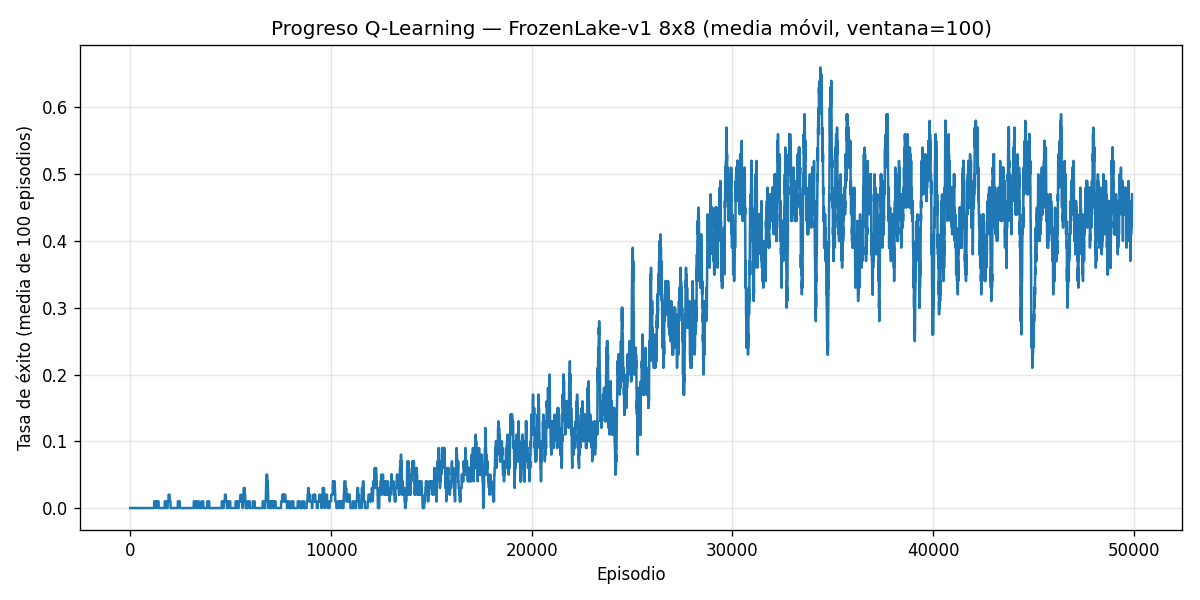
\includegraphics[width=0.78\textwidth]{q_learning_frozenlake.png}
\caption{Fase 1: media móvil (ventana 100) de la recompensa por episodio en
\code{FrozenLake-v1} 8$\times$8 resbaladiza. El aprendizaje despega hacia el episodio
$\sim$20k y se estabiliza en torno a 0.45--0.50.}
\label{fig:frozenlake}
\end{figure}

\section{Entorno, pipeline de visión y arquitectura}
\paragraph{Entorno.} Duckietown se ejecuta sobre la API de \code{gym} \emph{clásico}
(0.25.2), no Gymnasium, por compatibilidad con \code{gym-duckietown} (\code{daffy},
versión 6.1.34). \code{DuckieWrapper} (\code{src/wrappers.py}) adapta esa API antigua
(4-tupla) a Gymnasium (5-tupla) que espera Stable-Baselines3, y expone un espacio de acción
\emph{continuo}. La acción real del simulador son las \textbf{velocidades de las dos ruedas}
$[\,v_{\text{izq}}, v_{\text{der}}\,]\in[-1,1]^2$ (\code{action\_mode=wheels}); el agente las
produce directamente.

\paragraph{Pipeline de observación.} El procesamiento de cada observación es:
\[
\text{RGB }(480{\times}640{\times}3) \rightarrow \text{recorte 50\% superior (cielo)}
\rightarrow \text{grises} \rightarrow \text{resize }64{\times}64 \rightarrow (1,64,64)\ \texttt{uint8}
\]
y, tras \code{VecFrameStack(n\_stack=4)} (\code{src/envs.py}), $(4,64,64)$. El apilado de 4
frames da al agente percepción de velocidad y giro.

\paragraph{\texttt{CustomCNN}.} Extractor de características estilo \emph{NatureCNN}
(\code{src/cnn.py}): tres capas convolucionales
$\text{Conv}(32,8,4)\!\rightarrow\!\text{Conv}(64,4,2)\!\rightarrow\!\text{Conv}(64,3,1)$
con ReLU, \emph{flatten} y capa lineal a 256 características. \textbf{Importante:}
Stable-Baselines3 ya normaliza las imágenes \code{uint8} a $[0,1]$ (\code{normalize\_images}
por defecto) \emph{antes} de invocar el extractor, por lo que \code{CustomCNN} \textbf{no}
vuelve a dividir entre 255 (véase la Sección~\ref{sec:bugs}). Se conecta a SB3 vía
\code{policy\_kwargs} y es común a los tres algoritmos.

\section{Algoritmos}
\paragraph{DQN (baseline discreto).} Q-Learning profundo \emph{off-policy}. Como
Duckietown es continuo, \code{DiscreteActionWrapper} expone 5 acciones discretas mapeadas a
comandos de control. Config.: \code{lr}$=10^{-4}$, \code{buffer}$=50$k,
\code{learning\_starts}$=10$k, \code{batch}$=32$, \code{train\_freq}$=4$,
\code{target\_update}$=1000$, exploración $\varepsilon$ $1.0\!\rightarrow\!0.05$. Se discute
en la Sección~\ref{sec:bugs} una incoherencia detectada en su vocabulario de acción.

\paragraph{PPO (baseline continuo).} Gradiente de política \emph{on-policy} con
\emph{clipping}, estable y eficiente en muestras. Config.: \code{lr}$=3\cdot10^{-4}$,
\code{n\_steps}$=2048$, \code{batch}$=64$, \code{n\_epochs}$=10$, $\gamma=0.99$,
$\lambda_{\text{GAE}}=0.95$, \code{clip}$=0.2$. Es la base del modelo final.

\paragraph{SAC (algoritmo avanzado, Fase 3).} Actor-Crítico \emph{off-policy} de máxima
entropía, con exploración regulada automáticamente. Config.: \code{lr}$=3\cdot10^{-4}$,
\code{buffer}$=50$k, \code{batch}$=256$, $\tau=0.005$, \code{ent\_coef}=auto. Comparte
\code{CustomCNN} y wrappers con PPO.

\section{Metodología de entrenamiento e infraestructura}
El entrenamiento real se realizó en \textbf{Google Colab}. El stack de Duckietown exige
\textbf{Python 3.11} (incompatible con el kernel 3.12 de Colab), por lo que se monta un
\code{venv} 3.11 y se ejecuta todo como subproceso. Se resolvieron, de forma iterativa,
varios fallos nativos y de infraestructura:
\begin{itemize}
  \item \textbf{Dependencias:} \code{gym-duckietown} se instala con \code{--no-deps} y se
  re-fija \code{numpy==1.23.5} al final, para no romper el resto del stack.
  \item \textbf{Render headless:} \code{xvfb-run} + \code{MPLBACKEND=Agg}.
  \item \textbf{\emph{Segmentation fault} (Duckietown+OpenGL+SB3):} ocurría al
  \emph{inicializar} el modelo con el entorno real. La solución es el orden
  \textbf{\emph{model-first}}: construir el modelo sobre un entorno sintético con espacios
  idénticos y luego \code{model.set\_env(real)}. \code{train.py} y \code{eval.py} lo
  soportan con \code{--init-order model-first}.
\end{itemize}
El entorno real se confirma por consola:
\code{[duckie\_factory] Using real Duckietown env: Duckietown-loop\_empty-v0},
\code{gym-duckietown version 6.1.34}, \code{using DuckietownEnv}.

\section{Depuración: fallos que invalidaban los resultados}
\label{sec:bugs}
El hallazgo más relevante del proyecto es que varios resultados iniciales \emph{negativos}
no medían la calidad del agente, sino fallos del \emph{pipeline}. En orden de impacto:

\paragraph{(1) Caída silenciosa al \emph{mock}.} Si \code{gym\_duckietown} no se importaba o
no registraba sus entornos, la fábrica de entornos caía \emph{en silencio} a un
\code{MockDuckietownEnv} que devuelve \textbf{ruido aleatorio}. Todo lo entrenado/evaluado
así aprendía sobre ruido. Se corrigió \code{duckie\_factory.py} para (i) \textbf{fallar de
forma explícita} (\code{RuntimeError}) cuando se pide entorno real y no está disponible
---nunca cae al \emph{mock} con \code{use\_mock=False}--- y (ii) \textbf{importar
\code{gym\_duckietown} antes de \code{gym.make}} (ese import es lo que registra los IDs).

\paragraph{(2) Vídeo de render incorrecto.} \code{render()} devolvía un framebuffer ruidoso
bajo Xvfb y esta versión de \code{gym\_duckietown} no expone \code{render\_obs()}. La fuente
fiable de imagen es la \textbf{observación RGB cruda} del simulador, que \code{DuckieWrapper}
guarda en \code{last\_rgb\_frame} (\code{--video-source wrapper\_rgb}). Esto solo afecta a la
visualización, no a lo que ve el agente. Se confirma con
\code{frame source=venv.envs[0].last\_rgb\_frame | shape=(480, 640, 3)}.

\paragraph{(3) Convención de acción del baseline antiguo.} El baseline anterior solo conducía
bien con una transformación \emph{swap-negate} de la acción (\code{action\_mode=wheels\_fixed}):
su política quedó acoplada a una convención de ruedas concreta. Para un agente \emph{entrenado
desde cero} la convención es indiferente (el agente aprende el signo que recibe recompensa);
solo importa para \emph{reutilizar} el baseline antiguo. El modelo final se entrena con
\code{action\_mode=wheels} (por defecto) y, por tanto, \textbf{no} requiere ningún truco de
acción en evaluación.

\paragraph{(4) Doble normalización en la CNN (crítico).} \code{CustomCNN.forward} dividía la
entrada entre 255, pero SB3 \textbf{ya} normaliza las imágenes \code{uint8} a $[0,1]$ con
\code{preprocess\_obs(normalize\_images=True)} antes de llamar al extractor. Resultado: la
CNN recibía valores en $[0,\,1/255]\approx[0,\,0.004]$, unas \textbf{255 veces} más pequeños
de lo debido, degradando gravemente el aprendizaje de \emph{todos} los algoritmos. Verificado
en Colab:
\begin{verbatim}
preprocess_obs max: 0.7843137...   # SB3 ya normaliza a [0,1]
after extra /255 max: 0.0030757... # la CNN recibia ~255x menos senal
\end{verbatim}
\textbf{Corrección} (\code{src/cnn.py}): eliminar la división extra, dejando
\code{x = observations.float()}. Este fue el cambio decisivo: con la CNN corregida el
entrenamiento empieza a producir episodios completos con recompensa positiva.

\paragraph{(5) Vocabulario discreto incoherente en DQN.} Las acciones discretas
(\code{config.DISCRETE\_ACTIONS}) se diseñaron con semántica $[v,\delta]$ (velocidad, giro),
pero \code{DuckieWrapper} en \code{action\_mode=wheels} las interpreta como
$[v_{\text{izq}},v_{\text{der}}]$. Así, la acción ``recto'' $[0.6, 0.0]$ se ejecuta como
rueda izquierda 0.6 / derecha 0.0, es decir, un giro brusco: \textbf{DQN carece de una acción
de avance recto real}. Por ello DQN se reporta como \textbf{baseline sospechoso/descartado},
no como modelo final.

\section{Experimentos descartados (no entregables)}
\label{sec:descartes}
Por exhaustividad se probaron \emph{action modes} que reducen la dificultad inyectando
conocimiento de conducción. \textbf{Ninguno se entrega}, porque dejan de ser RL puro:
\begin{itemize}
  \item \code{safe\_discrete}: 5 maniobras de rueda predefinidas (recto/giros suaves). Es un
  \emph{prior} de control hecho a mano.
  \item \code{v\_omega\_safe}: $[v,\omega]$ con $v$ acotado a $[0.10,0.25]$ y $\omega$ limitado.
  Restringe a mano la dinámica para no salirse.
  \item \code{forward\_turn} (avance forzado): \textbf{no se implementó}; sería avance
  impuesto, no aprendido.
\end{itemize}
Igualmente se descartan controladores, PID y cualquier heurística de conducción. El
entregable usa \code{action\_mode=wheels} (acción de rueda directa, sin acotar).

\section{Resultados}
Todas las evaluaciones de esta sección usan la infraestructura \textbf{corregida} (entorno
real con fallo explícito, \code{model-first}); las cifras positivas reportadas en
iteraciones anteriores, previas a estos arreglos, no se reproducían y quedan
\emph{superadas}. La métrica principal es la recompensa media en el mapa oculto
\code{loop\_obstacles} (solo evaluación). La columna ``mejor \emph{rollout}'' es el de mayor
recompensa de un \emph{best-of-10} cualitativo en \code{loop\_obstacles}.

\begin{table}[h]
\centering
\footnotesize
\setlength{\tabcolsep}{4pt}
\begin{tabular}{lrrl}
\toprule
\textbf{Modelo} & \textbf{loop\_obstacles (media\,$\pm$\,std / len)} & \textbf{mejor rollout} & \textbf{decisión} \\
\midrule
Baseline antiguo + \code{wheels\_fixed} & $-869.9 \pm 548.6\ /\ 1264$ & --- & fallback inicial \\
PPO 20k \emph{(bug CNN)}      & $-924.2 \pm 441.4$ & --- & no supera baseline \\
DQN 20k \emph{(bug CNN)}      & $-1004.6 \pm 30.0$ & --- & descartado (Secc.~\ref{sec:bugs}) \\
SAC 20k \emph{(bug CNN)}      & $-1021.7 \pm 81.4$ & --- & no supera baseline \\
PPO 50k single-map \emph{(pre-fix)} & $-1481.8 \pm 473.3\ /\ 456$ & --- & más pasos no ayudan \\
PPO multimap 50k \emph{(pre-fix)}   & $-1764.9 \pm 712.8\ /\ 460$ & $-887.8$ & multimap no ayuda \\
\midrule
PPO \textbf{cnn-fix} 50k      & $-2038.0 \pm 1408.0\ /\ 1172$ & $\mathbf{1225.7}$ & rollouts positivos, alta varianza \\
\textbf{PPO cnn-fix 100k (ft)} & $\mathbf{-487.6 \pm 1049.9\ /\ 742}$ & $\mathbf{1249.5}$ & \textbf{MODELO FINAL} \\
\bottomrule
\end{tabular}
\caption{Evaluación en el mapa oculto \code{loop\_obstacles} (solo evaluación, nunca
entrenamiento). ``cnn-fix'' = con la doble normalización corregida. El modelo final
(\code{ppo\_cnnfix\_loop\_empty\_100k\_ft} $\rightarrow$ \code{best\_agent.zip}) tiene la
mejor recompensa media de la familia corregida y supera al baseline antiguo
($-487.6$ vs $-869.9$), con varios episodios completos de recompensa positiva (mejor
\emph{rollout} $1249.5$). La media negativa con \emph{std} alta refleja la elevada varianza
entre \emph{resets}.}
\label{tab:res}
\end{table}

\section{Discusión}
\textbf{El cambio decisivo fue corregir la normalización.} Antes del \emph{fix}, ningún
algoritmo (PPO/DQN/SAC, 20k o 50k, single o multimap) superaba al baseline: todos rondaban
$-900$ a $-1800$ en \code{loop\_obstacles}. Con la CNN corregida, el mismo PPO empieza a
generar episodios completos con recompensa positiva (mejor \emph{rollout} $1225.7$ ya a 50k).

\textbf{Por qué el modelo final es PPO cnn-fix 100k (fine-tuning).} Partiendo del PPO cnn-fix
50k se afinaron 50k pasos adicionales (RL puro, \code{lr} reducido, entrenamiento solo en
\code{loop\_empty}). Sube la recompensa media en \code{loop\_obstacles} de $-2038$ a $-487.6$
y mantiene el mejor \emph{rollout} en torno a $1250$. Es el mejor compromiso disponible:
mejor media que el baseline antiguo y mejor que cualquier variante anterior al \emph{fix}.

\textbf{Alta varianza.} La \emph{std} ($\pm1050$) y el \emph{best-of-10} (rollouts de $+1249$
a $-1397$, algunos terminando pronto) muestran que el agente conduce bien \emph{a veces} y se
sale otras según la pose inicial. Es una limitación real, no un artefacto de medida.

\textbf{DQN.} Se entrenó y evaluó, pero su vocabulario de acción no contiene un avance recto
real (Secc.~\ref{sec:bugs}, punto 5); queda como baseline \textbf{sospechoso/descartado}, no
como entregable.

\textbf{Pureza del enfoque.} El modelo final no usa \code{safe\_discrete}, \code{v\_omega\_safe},
\code{forward\_turn}, PID ni controladores: aprende de la imagen a velocidades de rueda
directas. Esas variantes se exploraron y se descartan por inyectar conocimiento de conducción.

\section{Conclusión}
La contribución práctica principal fue \textbf{diagnosticar y corregir} los fallos que
invalidaban silenciosamente el entrenamiento ---\emph{mock} silencioso, vídeo de render,
convención de acción y, sobre todo, la \textbf{doble normalización de la CNN}--- y, sobre la
base ya sana, entrenar un \textbf{PPO de RL puro} (50k + fine-tuning a 100k) que supera al
baseline anterior en el mapa oculto y produce conducción real en varios episodios. El modelo
final entregado es \code{best\_agent.zip} (copia de
\code{ppo\_cnnfix\_loop\_empty\_100k\_ft.zip}), evaluable sin ningún truco de acción.

\paragraph{Limitaciones y trabajo futuro.}
\begin{itemize}
  \item \textbf{Alta varianza} entre \emph{resets}: el desempeño depende mucho de la pose
  inicial. Mitigable con más pasos y/o evaluación más amplia.
  \item \textbf{Presupuesto de entrenamiento limitado} (50k--100k pasos): el RL desde píxeles
  en Duckietown suele requerir órdenes de magnitud más. \textbf{Futuro:} entrenar
  $\geq$300k--1M pasos con \textbf{vectorización real} (\code{SubprocVecEnv}, varios entornos
  en paralelo) para hacerlo viable en tiempo.
  \item \code{loop\_obstacles} es \textbf{más difícil} (obstáculos) y \textbf{solo de
  evaluación}: parte de la recompensa negativa es \emph{distribution shift} esperado.
  \item \textbf{Ajuste de hiperparámetros} (p.\,ej.\ \code{ent\_coef}$>0$ para más
  exploración) y \textbf{revisar el vocabulario de DQN} (incluir un avance recto real, o
  alinear la semántica con un \emph{action mode} coherente).
  \item Envolver la evaluación con \textbf{\code{Monitor}} para métricas de episodio más
  limpias.
\end{itemize}

\section*{Reproducibilidad}
Dependencias: \code{requirements.txt} (stack exacto, \code{stable-baselines3==2.2.1},
\code{gymnasium==0.29.1}, \code{gym==0.25.2}, \code{torch==2.12.0}) + \code{gym-duckietown}
aparte (\code{--no-deps}) + re-fijado de \code{numpy==1.23.5} (detalle en
\code{COLAB\_SETUP.md}). Protocolo y tabla de experimentos en \code{EXPERIMENTS.md}. El
modelo final se entrenó con \code{action\_mode=wheels} y se evalúa \emph{sin} \code{--action-mode}.
\begin{verbatim}
# Modelo final: PPO cnn-fix 50k + fine-tuning a 100k (RL puro, action_mode=wheels)
python train.py --algo ppo --map Duckietown-loop_empty-v0 --timesteps 50000 \
    --output ppo_cnnfix_loop_empty_50k --init-order model-first
python train.py --algo ppo --map Duckietown-loop_empty-v0 --timesteps 50000 \
    --output ppo_cnnfix_loop_empty_100k_ft \
    --init-model models/ppo_cnnfix_loop_empty_50k --learning-rate-override 5e-5 \
    --init-order model-first

# Evaluacion del modelo final en el mapa oculto (SOLO evaluacion)
python eval.py --algo ppo --model best_agent.zip \
    --map Duckietown-loop_obstacles-v0 --allow-eval \
    --init-order model-first --device cpu

# Video (camara real del robot)
python scripts/make_eval_video.py --algo ppo --model best_agent.zip \
    --map Duckietown-loop_obstacles-v0 --allow-eval \
    --video-source wrapper_rgb --rollouts 10 --init-order model-first
\end{verbatim}

\end{document}
